%%%%%%%%%%%%%%%%%%%%%%%%%%%%%%%%%%%%%%%%%%%%%%%%%%%%%%%%%%%% 
% This is the official template for theses and seminar papers from the Chair for Information Systems for Sustainable Society (IS3) at the University of Cologne

%
%PREAMBLE
%%%%%%%%%%%%%%%%%%%%%%%%%%%%%%%%%%%%%%%%%%%%%%%%%%%%%%%%%%%%%

\documentclass[a4paper, oneside, 12pt]{article}
\usepackage[utf8]{inputenc}
\usepackage[T1]{fontenc}
\usepackage{graphicx}
\usepackage{longtable}
\usepackage{hyperref}
\usepackage{caption}

% set margins for double-sided printing
\usepackage[left=2.5cm, right=2.5cm, top=2.5cm, bottom=2.5cm, bindingoffset=1.5cm, head=15pt]{geometry} 
\usepackage{setspace}
\onehalfspacing
% set headers
\usepackage{fancyhdr}
\pagestyle{fancy}
\fancyhead{}
\fancyfoot{}
\fancyhead[L,RO]{\textsl{\leftmark}}
\fancyhead[R,LO]{\thesisauthor}
\fancyfoot[C]{\thepage}
\renewcommand{\headrulewidth}{0.4pt}
\renewcommand{\footrulewidth}{0pt}

% set APA citation style
\usepackage{apacite}
\usepackage[numbib,notlof,notlot,nottoc]{tocbibind}
\pagenumbering{gobble}

%%%%%%%%%%%%%%%%%%%%%%%%%%%%%%%%%%%%%%%%%%%%%%%%%%%%%%%%%%%%%
%THESIS Parameters 
%%%%%%%%%%%%%%%%%%%%%%%%%%%%%%%%%%%%%%%%%%%%%%%%%%%%%%%%%%%%%

\title{Using discrete event simulation to test the feasibility of a vehicle choice model for on-demand car-sharing platform - Even wordier subtitle}

\newcommand{\thesisdate}{January 23rd, 2022}
\newcommand{\thesisauthor}{Luca Elias Fanselau} %input name
\newcommand{\studentID}{7369806} %input student ID
\newcommand{\thesistype}{Seminar Paper} % Set either to Bachelor or Master
\newcommand{\supervisor}{Univ.-Prof. Dr. Wolfgang Ketter}
\newcommand{\cosupervisor}{Muhammed Demircan}

%%%%%%%%%%%%%%%%%%%%%%%%%%%%%%%%%%%%%%%%%%%%%%%%%%%%%%%%%%%%%
%DOCUMENT
%%%%%%%%%%%%%%%%%%%%%%%%%%%%%%%%%%%%%%%%%%%%%%%%%%%%%%%%%%%%%

\begin{document}

%%%%%%%%%%%%%%%%%%%%%%%%%%%%%%%%%%%%%%%%%%%%%%%%%%%%%%%%%%%%%
%TITLE PAGE (Pre-defined, just change parameters above)
%%%%%%%%%%%%%%%%%%%%%%%%%%%%%%%%%%%%%%%%%%%%%%%%%%%%%%%%%%%%%
%%%%%%%%%%%%%%%%%%%%%%%%%%%%%%%%%%%%%%%%%%%%%%%%%%%%%%%%%%%%%
%TITLE PAGE
%%%%%%%%%%%%%%%%%%%%%%%%%%%%%%%%%%%%%%%%%%%%%%%%%%%%%%%%%%%%%
\makeatletter
\begin{titlepage}
    \begin{center}
        \vspace*{1cm}

        \Large
        \textbf{\@title}

        \vspace{1.5cm}
        
        \thesistype{}
        
        \vspace{1cm}

        \begin{figure}[htbp]
             \centering
             
\includegraphics[width=.5\linewidth]{./Figures/UoC_Logo.png}
        \end{figure}

        \vspace{1cm}

        \large
        \textbf{Author}: \thesisauthor{} (Student ID: \studentID{})\\
        \large
        \textbf{Supervisor}: \supervisor{}\\
        \large
        \textbf{Co-Supervisor}: \cosupervisor{}

        \vspace{1cm}
        \large
        Department of Information Systems for Sustainable Society\\
        Faculty of Management, Economics and Social Sciences\\
        University of Cologne\\

        \vspace{1cm}
        \@date

    \end{center}
\end{titlepage}
\makeatother

%%%%%%%%%%%%%%%%%%%%%%%%%%%%%%%%%%%%%%%%%%%%%%%%%%%%%%%%%%%%%
%SOOA
%%%%%%%%%%%%%%%%%%%%%%%%%%%%%%%%%%%%%%%%%%%%%%%%%%%%%%%%%%%%%
\clearpage
\thispagestyle{empty}
\section*{Eidesstattliche Versicherung}
\label{sec:SOOA}

\vspace{2.5cm}

% Statement of original authorship - Needs to be in German
% see also here: https://www.wiso.uni-koeln.de/sites/fakultaet/dokumente/PA/formulare/eidesstattliche_erklaerung.pdf

Hiermit versichere ich an Eides statt, dass ich die vorliegende Arbeit selbstständig und ohne die Benutzung anderer als der angegebenen Hilfsmittel angefertigt habe. Alle Stellen, die wörtlich oder sinngemäß aus veröffentlichten und nicht veröffentlichten Schriften entnommen wurden, sind als solche kenntlich gemacht. Die Arbeit ist in gleicher oder ähnlicher Form oder auszugsweise im Rahmen einer anderen Prüfung noch nicht vorgelegt worden. Ich versichere, dass die eingereichte elektronische Fassung der eingereichten Druckfassung vollständig entspricht.

\vspace{1cm}

\noindent
Die Strafbarkeit einer falschen eidesstattlichen Versicherung ist mir bekannt, namentlich die Strafandrohung gemäß § 156 StGB bis zu drei Jahren Freiheitsstrafe oder Geldstrafe bei vorsätzlicher Begehung der Tat bzw. gemäß § 161 Abs. 1 StGB bis zu einem Jahr Freiheitsstrafe oder Geldstrafe bei fahrlässiger Begehung.

\vspace{3cm}
\noindent
\textbf{\thesisauthor{}} 

\vspace{0.5cm}
\noindent
Köln, den xx.xx.20xx


%%%%%%%%%%%%%%%%%%%%%%%%%%%%%%%%%%%%%%%%%%%%%%%%%%%%%%%%%%%%%
%ABSTRACT
%%%%%%%%%%%%%%%%%%%%%%%%%%%%%%%%%%%%%%%%%%%%%%%%%%%%%%%%%%%%%
\clearpage
\thispagestyle{empty}
\section*{Abstract}



%%%%%%%%%%%%%%%%%%%%%%%%%%%%%%%%%%%%%%%%%%%%%%%%%%%%%%%%%%%%%
%TOC,TOF,TOT
%%%%%%%%%%%%%%%%%%%%%%%%%%%%%%%%%%%%%%%%%%%%%%%%%%%%%%%%%%%%%
\clearpage
\pagenumbering{Roman}
\tableofcontents
\clearpage
\listoffigures
\clearpage
\listoftables
\clearpage

\pagenumbering{arabic}


%%%%%%%%%%%%%%%%%%%%%%%%%%%%%%%%%%%%%%%%%%%%%%%%%%%%%%%%%%%%%
%MAIN PART
%%%%%%%%%%%%%%%%%%%%%%%%%%%%%%%%%%%%%%%%%%%%%%%%%%%%%%%%%%%%%

% Introduction
\clearpage
\section{Introduction}
\label{sec:Intro}

Car sharing services have recently seen a rapid rise in popularity 
and valuations of the global car-sharing market expect to grow to
a total value of USD 6.5 billion by 2024, from just USD 1.1 billion in 2015 \shortcite[p.~1]{Emissions2018}. 
A primary reason for that is the high value-proposition a car-sharing service
can offer to its customers. This includes positive environmental impact in the form of
reduced individual CO2 emission by up to 312 kg CO2 / year, as well as
lower individual mobility costs, compared to owning a vehicle \shortcite[p.~1525]{UlmEnv2011}. Together with the
broad adoption of smartphones equipped with apps, that typically
support the reservation and operation of shared vehicles, Car Sharing Organizations (CSOs)
can provide an appealing alternative to other public or private transportation measures.

These services can be categorized into free-floating, meaning vehicles of the fleet
can travel freely in a restricted area, and non-floating systems, where vehicles must travel
between discrete stations that typically offer a fixed amount of spaces. Additionally,
there is also a distinction between one-way and two-way car-sharing systems, the former
describes services where the user can travel from point A to point B, which he can choose
freely, while the latter expects the user to return the vehicle to the spot where it was
rented.

Operating large scale on-demand car-sharing networks tends to be difficult, since
deploying operational decision is often bound to large expenses and, especially if the
system is already in use, can not be done in a trial and error fashion. One way to test the feasibility of
seemingly optimal proposals rapidly is to develop a simulation which tries to capture the real world
interaction of actors in a car sharing network to a sufficient degree. With this an operator can 
quickly assess if the solution holds up to various real world restrictions that are characteristic
for car sharing networks, such as demand served or, in the case of an EV car-sharing platform, the vehicle
charge levels \shortcite[p.~224]{OptSimFramework}

The focus of this seminar thesis is firstly, to analyze existing literature on CSOs and especially
the use of simulation environments and the optimization problems that were solved using them.
Secondly, to use that information to design
and implement a discrete event simulation, that models a non-floating one-way on-demand
car-sharing service. This simulation is then equipped with a vehicle choice
classifier model, based on socio-demographic and request specific features,
to model the real world mobility dynamics of a car-sharing network.
The main objective of the proposed framework is to use metrics obtained by the simulation
to study the impact of fleet size and Substitution effects on overall performance.


% Literature Review
\clearpage
\section{Literature Review}
\label{sec:lr}
...
\subsection{Exemplary Figure}
\label{subsec:Section_Name/fig}
...
\begin{figure}[htbp]
    \centering
    
\includegraphics[width=.5\linewidth]{./Figures/UoC_Logo.png}
    \caption{Exemplary Figure}
    \label{fig:UoC}
\end{figure}


\subsection{Exemplary Figure Referencing}
\label{subsec:Section_Name/fig_rfs}

See Figure \ref{fig:UoC} for details. Additional information can be
found in the footnote \footnote{Image taken from \url{https://en.wikipedia.org/wiki/File:Siegel_Uni-Koeln_(Grau).svg}.}.


% Simulation
\clearpage
\section{Simulation}
\label{sec:Simulation}

\subsection{Model Restrictions}
\label{subsec:Simulation/restrictions}


% Vehicle Choice Model
\clearpage
\section{Vehicle Choice Model}
\label{sec:ChoiceModel}

Mathematical description of vehicle choice model

% Maybe a model that calculates if a vehicle will be rented
Palette: https://flatuicolors.com/palette/ru


\subsection{Data source}
\label{sub_sec:DataSource}

- Dataset 4gb
- Zensus data


\subsection{Data preparation}
\label{sub_sec:DataPreparation}

- Huge bias towards smart fourtwo
- Missing income
- 


\begin{itemize}
  \item House hold -> Size relation
  \item College to size -> No real thingy
  % \item Dataset: https://www.kaggle.com/steventaylor11/stated-preferences-for-car-choice
\end{itemize}

Features:

We propose a person, which is defined by a feature vector. From now on a person strictly refers to a specific realization 
of these features unless mentioned otherwise. 

\begin{longtable}{l | c}
  \caption{Features}
  \label{table:features}
  \\
  \textbf{Label} & \textbf{Description} \\
  \hline
  age & The current age of this person, must be > 18 years. unbounded otherwise \\
  hss & Household size\\
  college & 1 (or true) if the person had college education, 0 (or false) otherwise \\
  income & Monthly income, before taxes \\
  comm & Commuting distance (daily)
\end{longtable}

Scoring algorithm with the following "decisions":

Early opt out case: $age < 21$: Typically only the XS category is allowed to be driven by persons under the age of 21.
Otherwise we will employ a scoring algorithm which, where we calculate a score $s(o)$ where 
$o \in \{ \textrm{XS}, \textrm{S}, \textrm{M}, \textrm{L} \} = C$. The score is based on various sub-scores, namely:
$$
s_0(o) = 
\begin{cases}
  1 - P(\text{hss} > 2 \land \text{category} = o), & \text{if}\ \text{hss}\ \le 2 \\
  P(\text{hss} > 2 \land \text{category} = o), & \text{otherwise}
\end{cases}
$$
where $P(\text{hss} > 2 \land \text{category} = o) \ \forall o \in C$ is determined empirically by using the data source 
mentioned in \ref{sub_sec:DataSource} and can be found in the Appendix\todo{Add that to the Appendix}. Another important 
scoring mechanism depictures a correlation between commuting distance and the size an can be similarily described as:
$$
s_1(o) = 
\begin{cases}
  1 - P(\text{comm} > 2 \land \text{category} = o), & \text{if}\ \text{hss}\ \le 2 \\
  P(\text{comm} > 2 \land \text{category} = o), & \text{otherwise}
\end{cases}
$$



% Results & Discussion
\clearpage
\section{Results \& Discussion}
\label{sec:Results}


Succeeding the implementation phase the results of the simulation framework had to be analyzed. Due
to the complexity and high dimensionality of the problem, a focus was made on the effects of the parameters
$C$ and $\alpha$ on the metrics defined in section \ref{sub_sec:Method/Metrics}.

\subsection{Simulation Result}
\label{sub_sec:Results/Results}

\begin{figure}[htbp]
  \centering
  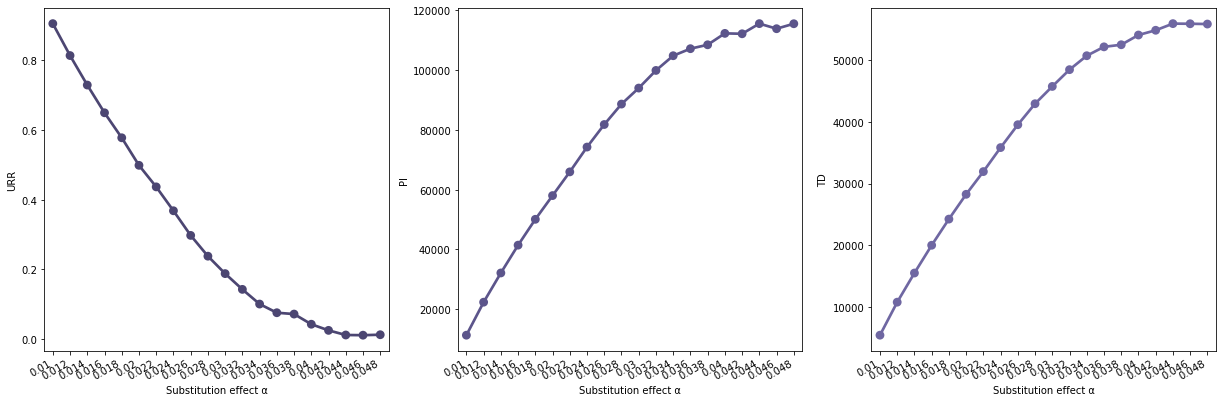
\includegraphics[width=\linewidth]{./Figures/alpha.png}
  \caption{Effects of alpha for performance metrics}
  \label{fig:Alpha}
\end{figure}

Starting with the effect of the substitution effect $\alpha$. The Figure \ref{fig:Alpha} shows the
metrics defined in Section \ref{sub_sec:Method/Metrics} in order. For this evaluation the capacity
was set to $C = 5$, leading to a higher importance of the substitution effect. A clear dependency
of the value of alpha to a higher performing car-sharing network can be seen. However, the curves
also indicate that the impact of the parameter decreases with larger values and the random
signal, that is due to the random nature of the simulation environment, increases.

\begin{figure}[htbp]
  \centering
  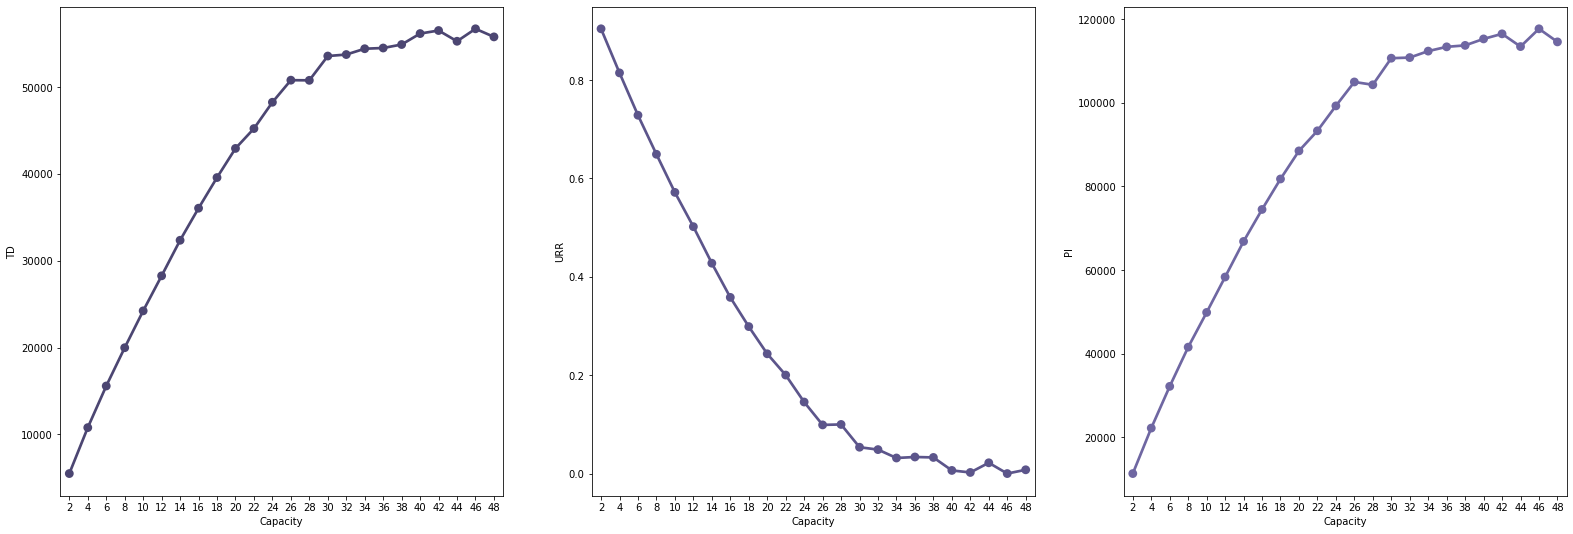
\includegraphics[width=\linewidth]{./Figures/capacity.png}
  \caption{Effects of capacity for performance metrics}
  \label{fig:Capacity}
\end{figure}

A very similar effect can be seen in Figure \ref{fig:Capacity} with the parameter $C$,
the capacity at each station. For these the alpha value has been set to $\alpha = 0.05$,
the optimal value based on previous results. From an operational standpoint an optimal
fleet capacity could be determined by averaging the metrics over multiple runs
and define a threshold below which the increase in overall performance with regard to the
increase in fleet size provides no added value to the network. This effect was also discovered
by \shortciteA{Nourinejad2014}.

\begin{figure}[htbp]
  \centering
  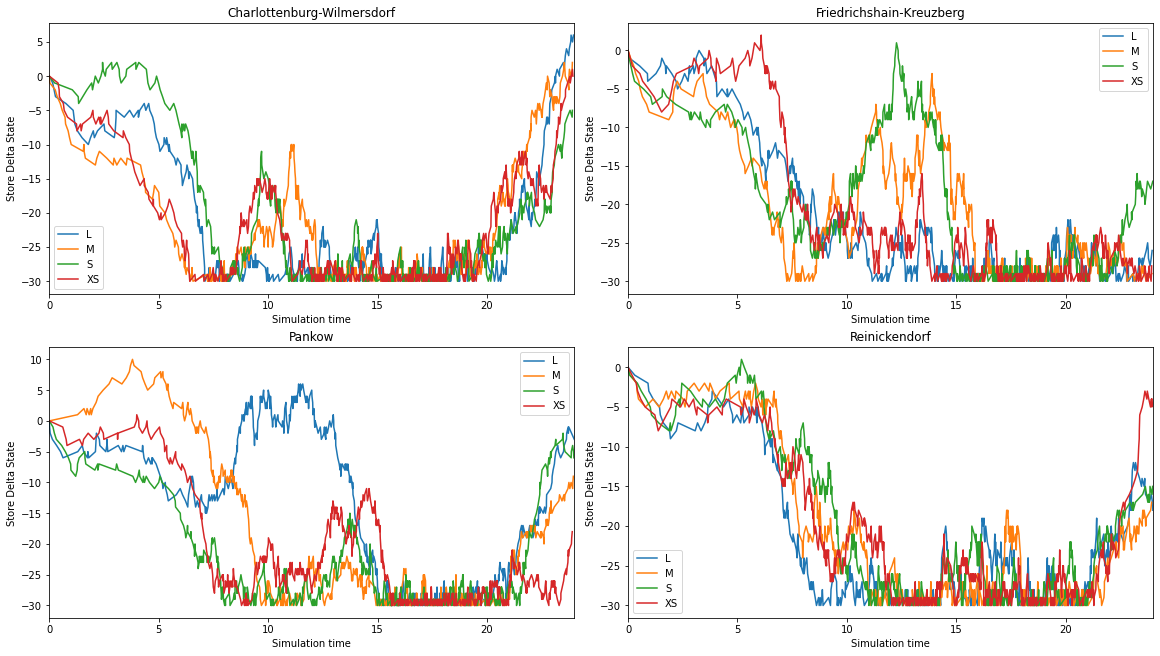
\includegraphics[width=\linewidth]{./Figures/delta-func.png}
  \caption{$\Delta_s(t, c)$ for a simulation with $\alpha=0.003, C=30$}
  \label{fig:DeltaFunc}
\end{figure}

Lastly the state function of the stations $\Delta_s(t, c)$ has been plotted against the
simulation time, to get insights of the state at each station throughout the working day.
As can be seen in Figure \ref{fig:DeltaFunc}, the impact of the demand described in Figure \ref{fig:Demand}
is clearly visible. Especially during the rush hour in the late afternoon all stations
reach capacity limits, but just about manage to keep up with an unsatisfied customer rate (URR)
of just 6.50\%. 

\subsection{Discussion \& Further Research}
\label{sub_sec:Results/Discussion}

As mentioned previously the topic of simulation in a large scale network, like a car-sharing network,
is a problem with high-dimensionality, therefore providing a lot of potential further research areas.
The focus of this thesis also included to make the simulation environment as general 
as possible, such that additional research could be conducted on the same code base.

One aspect that could be of interest, is the selection of start and end stations for
each customer request. In the real world this is typically not equally distributed but
often follows traffic flows, which are among others time and location dependent.
Another potential extension, could include an increased set of stations $\mathbb{S}$ to
study even larger car-sharing networks.

While training the classifier, it became apparent that the signal of the socio-demographic
data of the rental area only correlated loosely with the decision made, and feature importance
was quite low. In further research a more sophisticated classifier could be trained that
sources a dataset which directly correlates one rental to for example the age of the
customer. Due to the modularity of the simulation that model could then easily be
exchanged with the classifier trained in this thesis and used in the simulation 
environment. 

Another aspect that would be of particular interest for the simulation stage is the parameter
$\alpha$. This parameter is not controllable by the operator but inherent for a particular
customer group. One could convey a study to try to estimate the real world $\alpha$ for different
deployments of a car-sharing networks empirically.


% Conclusion
\clearpage
\section{Conclusion \& Further Research}
\label{sec:Conclusion}

\subsection{Exemplary Citation}
\label{subsec:Section_Name_X/cite}

% use \shortciteA when using author names in text

In this research we follow \shortciteA{Ketter2016}...

% use \shortcite to reference normally in brackets

PowerTAC is an example of a multiagent competitive gaming platform \shortcite{Ketter2016}.

%%%%%%%%%%%%%%%%%%%%%%%%%%%%%%%%%%%%%%%%%%%%%%%%%%%%%%%%%%%%%
%APPENDICES
%%%%%%%%%%%%%%%%%%%%%%%%%%%%%%%%%%%%%%%%%%%%%%%%%%%%%%%%%%%%%


\appendix
\renewcommand*{\thesection}{\Alph{section}}\textbf{}

% APPENDIX A
\clearpage
\section{Appendix}
\label{app:A}
...

%%%%%%%%%%%%%%%%%%%%%%%%%%%%%%%%%%%%%%%%%%%%%%%%%%%%%%%%%%%%%
%BIBLIOGRAPHY
%%%%%%%%%%%%%%%%%%%%%%%%%%%%%%%%%%%%%%%%%%%%%%%%%%%%%%%%%%%%%

\clearpage
\renewcommand*{\thesection}{}\textbf{}

\bibliographystyle{apacite}
\bibliography{Bibliography.bib}


\end{document}
